% !TEX root = main.tex

\chapter{はじめに}

% 多次元索引の概要・有用性
多次元索引は複数の次元で表されたキーによる検索を補助するデータ構造である.
地理情報システムにおける空間オブジェクトの検索や,データベース管理システムにおける多次元データの選択演算効率化などに利用される.
多次元データは複数の次元から成るが,メモリやストレージ上では1次元空間上に配置されるため,多次元空間上での局所性を適切に反映した索引構造が求められる.

% 多次元索引の種類
多次元索引は多次元空間を直接扱うものと1次元空間へ射影して扱うものの大きく2つに分けられ,本稿では後者を主に扱う.
多次元空間を直接扱う索引の代表例はR木~\cite{sigmod:Beckmann1990}であり,多次元の包囲矩形などを用いて多次元空間を階層的に分割していく.
1次元空間へ射影するものは主に空間充填曲線に基づいており,Universal B木(UB木)~\cite{wwca:Bayer1997}が代表である.
後者の利点は,既存の効率的な1次元索引を流用でき,挿入・削除に伴う木の構造変更などが容易な点である.
一方で欠点として,多次元データを1次元化するため,隣接するデータが多次元空間上では近接していない可能性がある点が挙げられる.

% UARTの提案と問題点
本稿ではUB木およびAdaptive Radix Tree(ART)~\cite{icde:Leis2013}を組み合せた索引構造であるUniversal ART(UART)~\cite{deim:Suzuki2023}の改善について述べる.
UARTは汎用的に使用可能な多次元索引だが,データに偏りがある場合に挿入と範囲検索の性能が低下するという課題を持つ.
性能低下の原因は,不適切な空間分割による疎な部分空間の生成である.
UARTではノードの空きスペースがなくなった際に対応する多次元空間を分割することでノードを分割するが,分割後の部分空間が十分な数のレコードを持つという保証がない.
そのため挿入されるレコードに空間的な偏りがある際に,レコードを少数しか持たない疎なノードが多数生成され性能を低下させている.

% 本論文の目的と論文構成
本研究では分割後の各空間が十分な数のレコードを持つよう空間分割の手法を改善する.
まず,UARTの基となるARTとUB木の概要について述べ,続けてUARTの概要について述べる.
最後に,既存手法における空間分割の問題点と空間使用量に基づく空間分割の改善について説明し,論文全体のまとめを述べる.




\chapter{関連研究}

UARTの構成要素として利用するUB木とARTについて説明する.

\section{Universal B木(UB木)}

UB木~\cite{vldb:ramsak2000}は,多次元空間を\ZCurve に基づき1次元空間に変換し,変換後の\ZValue を\BTree のキーとして使用する索引構造である.
構造自体と,検索・挿入・削除といった各操作は\BTree と変わらない.
そのため,UB木の特徴である\ZCurve と\BTree について述べる.

\ZCurve ~\cite{acm:Gaede1998}は空間充填曲線の一種であり,2次元空間であれば``Z''の記号を描くような曲線となる.
\ZValue は\ZCurve 上の開始点からの距離であり,距離が近いものは多次元空間上でも近いことが多い.
ただし,空間充填曲線の性質上,\ZValue としては隣接するものが多次元空間上では遠く離れる場合もある.
\ZValue への変換は,多次元座標の各座標を2進符号化し上位ビットから順に交互配置することで行う.

\BTree ~\cite{book:Kitagawa1996}は,\Fig{\ref{fig:bptree}}に示すように索引部とデータ部からなるバランス木である.
索引部はレコードのキー値とデータ部へのポインタが格納された中間ノードの集まりである.
一方,データ部はキー値に対応するレコードと,隣の葉ノードをつなぐポインタが格納された葉ノードの集まりである.
そのため,木の高さが葉ノードの広がりに比べ低くなりノードアクセス数が減少する.

以上の構造から,\BTree は読み取り操作(点検索および範囲検索)・書き込み操作両面においてバランスの取れた性能を持つ.
索引部がレコードそのもではなくキー値のみになっていることから,点検索におけるキー値の比較や書き込み操作による索引部の変更が効率よく行える.
更に,葉ノードのポインタをたどることで全検索や範囲検索も高速に行うことができる.
また,各ノードはが全て同じサイズの領域として管理されるのでメモリ管理が容易となり利用効率も向上する.

\begin{figure}[tb]
  \centering
  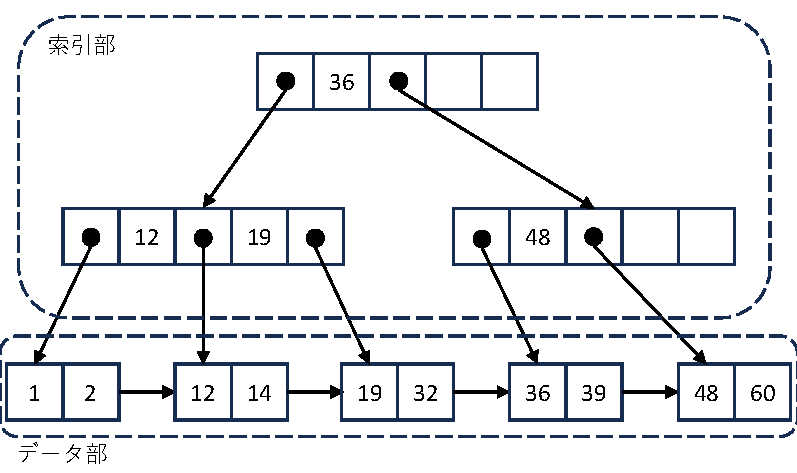
\includegraphics{./figures/fig_bptree.pdf}
  \caption{\BTree{}の構造}
  \label{fig:bptree}
\end{figure}

UB木は\BTree{}の一種であるためそのデータ構造は効率的だが,空間分割が非効率的であるという問題がある.
UB木はノードの空き容量がなくなった際にノードを分割するが,分割点は分割後のサイズによって決定され,空間的な面は基本的に考慮されない.
つまり,多次元空間上で非連続な領域が同じノードに割り当てられる可能性があり,各ノードに対応する多次元包囲矩形が過剰に拡大しうる.

\section{Adaptive Radix Tree(ART)}

ART~\cite{icde:Leis2013}は基数木(Radix Tree)の拡張であり,レコード数に応じてノードサイズを動的に選択する索引構造である.
また,基数木はトライ木の空間利用効率を最適化した索引構造である.
そのため,本節ではトライ木と基数木の概要について述べてから,動的選択の概要について述べる.

トライ木は,文字列を表すための索引構造である.
根ノード以外のノード一つ一つが1文字を表し,文字の種類数だけ子ノードへのポインタを持つ.
文字列は,根ノードから葉ノードまでに通ったノードの順で文字をつないだものである.

トライ木は,文字列の検索速度に優れるが,空間利用効率が非常に大きい.
全ての子ノードが文字の種類数だけポインタを持つため,文字の種類数が多かったり,文字列が長かったりすると非常に大量のメモリを消費する.
加えて,ポインタの多くがヌルポインタとなり空間利用効率も悪い.
そこで,トライ木の空間利用効率を抑えた索引構造が基数木である.

基数木は,基本的にトライ木と同様の索引構造である.
基数木とトライ木の違いは,子ノードが一つしかないノードをひとまとめにすることである.
つまり,ある文字の後に続く文字が1種類しかない場合は,ノードに文字列を対応させる.
まとめた文字が多いほど,ノードの数が減り空間使用量を抑えられる.
しかし,まだ多くのノードがヌルポインタを持つため空間利用効率はよくない.
そこで,大量のヌルポインタを減らした索引構造がARTである.

ARTでは与えられたキーを1バイトの部分キーに分割し索引を構築するため,各ノードで最大256個のレコードを保持する.
そこで,ヌルポインタの数を減らすために,子ノードの数に応じて使用するノードを変える.
選択されるノードはNode4,Node16,Node48,Node256の4種類であり,それぞれ対応する数のレコードを格納できる.
各ノードは保持するレコードの数だけでなく,保持する方法も違う.

Node4は,キーと子ノードへのポインタを4個ずつ持つ.
キーとキーに対応する子ノードへのポインタは,どちらも$i$番目に保持される.
ここで,キーが保存される配列を$key\_array$,ポインタが保存される配列を$pointer\_array$とすると,$key\_array[i]=key$,$pointer\_array[i]=child\_pointer$が成立する.
つまり,$i$番目のキーはi番目のポインタに対応している.
Node16もキーとと子ノードへのポインタを持つ数が16になっただけで,Node4と同じ構造である.

Node48は,キーと子ノードへのポインタを48個ずつ持つ.
しかし,$key\_array$のサイズは256である.
そして,キーの値がキーが格納されているインデックスの値と一致し,キーの値と対応する子ノードへのポインタが格納されているインデックスの値と一致する.
つまり,$key\_array[key]=i$,$pointer\_array[i]=child\_pointer$が成立する.

Node256では,キーと子ノードへのポインタを256個ずつ持つ.
$key\_array$はなく,キーが$pointer\_array$のインデックスに一致する.
つまり,$pointer\_array[key]=child\_pointer$が成立する.

ARTは部分キーに偏りのある箇所では容量の少ないNode4やNode16が使用され,基数木の欠点である空間利用効率の悪化を克服している.
UARTでもキーの管理にノード選択を用いることで空間利用効率を向上させている.




\chapter{Universal Adaptive Radix Tree(UART)}

UARTはUB木を拡張し,主に空間分割を担うART層と挿入されたレコードの保持を担うUB層に分けた多次元索引である.
\ZCurve は多次元空間を1次元上の値として表現しており,上位ビットから下位ビットに進むにつれ粒度の細かい空間分割が行われる.
そこで,UARTでは変換後の\ZValue を1バイトずつの部分キーに区切り,部分キーによって表される空間分割をARTにより管理する.
つまり,ART層では多次元空間上でレコードが密な領域ほど空間が分割され,深い階層が生成される.
UB層は挿入されたレコードを保持するデータ層であり,該当領域に存在する疎なレコード群への効率的な範囲走査を実現する.

\Fig{\ref{fig:uart}}にUARTの概念図を示す.
本来のUARTでは\ZValue を1バイトずつに区切るが,\Fig{\ref{fig:uart}}では\ZValue を4ビットごとに区切っている.
また,ART層の丸はレコードを,UB層の丸はUB木のノードを表している.
そして,区切られた\ZValue のうち上位4ビットと中位4ビットは各層のグレー色で塗りつぶされた区画に,下位の4ビットは最下層にある灰色のレコードに対応している.
以下では,ART層とUB層の構造について概略を述べる.

\begin{figure}[tb]
  \centering
  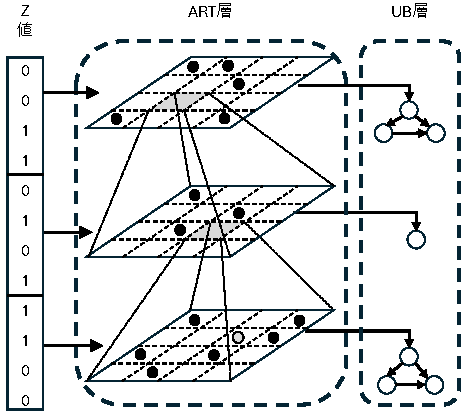
\includegraphics[scale = 1.75]{./figures/fig_uart.pdf}
  \caption{UARTの構造}
  \label{fig:uart}
\end{figure}

\paragraph{ART層}

ART層は\ZValue をキーとしてARTに格納することで多次元空間を階層的に分割する索引層である.
ARTではキーを1バイトの部分キーに分割するため,各階層で空間は256分割される.
分割された空間のうちレコードが密に存在する箇所は後述する手続きによって下の階層が生成され,再帰的により細かい空間分割が行われる.
一方,ART中の各ノードはUB木の根ノード(i.e., UB層へのポインタ)をヘッダ領域に持ち,下の階層を持たない空間のレコードはそちらで保持される.

\paragraph{UB層}

UB層はART層の各階層各空間で保持されるUB木の集合であり,レコードの実体はこちらで管理される.
各UB木はその階層における\ZValue の部分キーを検索キー,挿入された空間オブジェクトとペイロードの組をレコードとして持つ.
なお最下層,つまり\ZValue の全長を用いた空間分割後のUB木は,部分キーとなる\ZValue を持たないため一般的な\BTree として生成される.
UB木の構築方法は既存のものと同様であり,\BTree に由来する効率的な範囲走査を可能とする.
ただし,既存研究において各UB木は根ノードのみしか持たない点に注意する~\cite{deim:Suzuki2023}.





\chapter{UARTにおける空間分割の効率化}

既存研究の課題として,オブジェクトが疎に分布する空間の管理が不十分であり,偏った分布における性能低下が挙げられる~\cite{deim:Suzuki2023}.
例えば全オブジェクトが1つの部分空間に偏る場合は,最下層までARTが展開され,\BTree によって全オブジェクトが管理されるため空間効率に関する問題は発生しない.
同様に,オブジェクトが空間全域で一様に分布する場合は,各部分空間に対応するUB木が一定数のオブジェクトを管理するためこちらも問題ない.
しかし,分布が適度に偏っているとき,既存のUARTでは少数のレコードしか持たないUB木が多数生成され性能が低下してしまう.

分布の偏りによる性能低下は,既存研究におけるUB木が根ノード1つしか持たず,オブジェクトが疎な空間のレコードを十分に保持できないためである.
既存研究ではUB木の根ノードを一種の書込み用バッファとして利用しており,空き容量がなくなった際は即座にオブジェクト数が最も多い部分空間を選びART層で下層を生成する.
この密な空間を選ぶという方針自体は誤っていないが,部分空間における空間使用量を考慮せず,単純にレコード数の多い空間を選ぶという手続きに問題がある.
つまり,各部分空間のオブジェクト数の差が少ない(i.e., 分布がロングテールを持つ)とき,この手続きではオブジェクト数が少ない部分空間においても下層が生成されてしまう.
現実的なワークロードやデータセットにおいてロングテールは頻出するため,この問題への対応は必須である.

そこで本研究では,下層生成の条件として一定の空間使用量を持つことを使用し,UB層において根ノード単体ではなくUB木としてレコードを保持する.
UB木は\ZValue を使用した二次索引であり,同じ\ZValue を持つレコードは内部で転置リスト(posting list)として保持される.
既存研究では各転置リスト内のレコード数のみを見たが,本研究では転置リストのサイズも考慮し一定のサイズを超えるまで下層を生成しない.
つまり,ノードの空き容量がなく下層も生成しない場合はノードを分割し,UB木を拡張する.
これにより,生成された下層には一定以上のオブジェクトが必ず含まれるため,各ノードの空間利用効率およびそれに伴う範囲走査性能の向上が見込める.





\chapter{評価実験}

本章では,偏りなどデータのパラメータに対する頑健性と,実データを用いた有用性を評価する.
そのために,各データに対して読み込みと書き込みを行い,それぞれのスループットを測定する.
以下ではより詳細な実験方法について述べる.

本実験では,頑健性・有用性のどちらの評価においても,用意したデータに挿入,構築・破棄,範囲検索処理を行いスループットを測定する.
比較対象は既存手法のUARTと,多次元索引としてよく使われるUB木と\RTree である.
\RTree は空間利用効率が高く範囲検索に優れており,データの次元数に合わせてboostとlibspatialindexの2つの実装を用いる.
boostの実装が,libspatialindexの実装に比べ高速な一方で,4次元以上に対応していないためである.
どの実験も全て単一スレッドで行い,命令を逐次的に発行する.
\Tab{\ref{tab:environment}}に本実験で使用する環境を示す.

\begin{table}[tb]
  \caption{実験用サーバの構成}
  \label{tab:environment}
  \centering
  \begin{tabular}{ll}
    \toprule
    Item     & Value                                              \\
    \cmidrule(r){1-1}
    \cmidrule(l){2-2}
    CPU      & Intel(R) Xeon(R) Gold 6262V (two sockets)          \\
    RAM      & DIMM DDR4 (Registered) 2933 MHz (16GB $\times$ 14) \\
    OS       & Ubuntu 22.04.2 LTS                                 \\
    Compiler & GNU C++ ver. 9.4.0                                 \\
    \bottomrule
  \end{tabular}
\end{table}

そして,有用性の評価には,日本,アジア,地球の規模の異なる3つの地理データセットを用いる.
また,パラメータに対する頑健性の評価には,各次元の値がZipf関数に従うシミュレーションデータを用いる.

Zipf関数は各次元の値がZipfの法則に従うように多次元値を生成する関数である.
Zipfの法則は,ある要素の出現頻度とその大きさに双曲線の関係が成り立つという経験則である.
そして,Zipfデータセットは各次元独立で近似的に\Eq{\ref{eq:zipf}}に示すZipf分布に従う\footnote{\footnotesize\url{https://github.com/dbgroup-nagoya-u/cpp-utility}}.
\begin{equation}
  \label{eq:zipf}
  f(k; \alpha, |W|) = \frac{1 / k^{\alpha}}{\sum_{n = 1}^{|W|} 1 / n^{\alpha}}
\end{equation}
\Eq{\ref{eq:zipf}}中の\alpha はスキューパラメータであり,$\alpha = 0$の時にZipfデータセットは一様分布となる.

\section{ページサイズ}
UARTのハイパラメータに葉ノードのページサイズがある.
ページサイズはレコードの容量として捉えられるため,挿入操作や範囲検索の結果を左右することが容易に考えられる.
そこで,UARTとその他の索引構造との比較する前に,UARTの改善後と改善前においてページサイズが各性能に与える影響を評価する.

UARTの改善前後で挿入と範囲検索のスループットを測定した.
以降では,UARTの改善後をUART(改善後),UARTの改善前をUARTと表記する.
UART(改善後)は全てのページサイズにおいてUARTよりよい結果が得られた.
挿入では,UART(改善後)はUARTの1.3倍から1.8倍ほどのスループットになった.
UART(改善後)ではページサイズの影響が小さく,UARTではページサイズが大きくなるとスループットが小さくなった.
また範囲検索では,UART(改善後)はUARTの1.5倍から1.9倍ほどのスループットになった.
挿入のときとは反対に,UART(改善後)ではページサイズが大きくなるとスループットも大きくなり,UARTではページサイズの影響が小さかった.
結果を\Fig{\ref{graph:pagesize}}に示す.
\begin{figure}[tb]
  \centering
  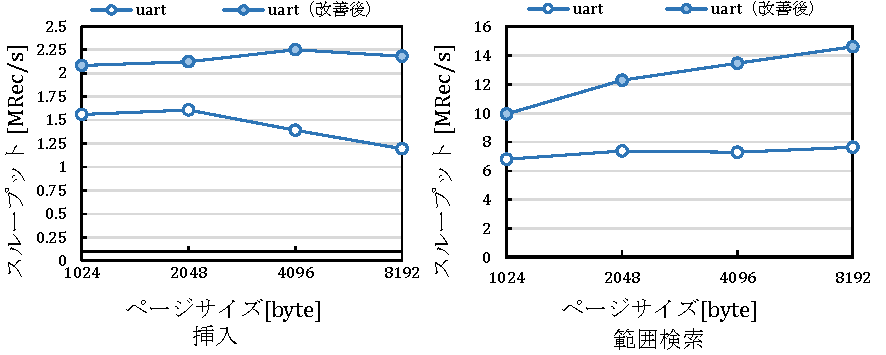
\includegraphics{./figures/graph-pagesize.pdf}
  \caption{UARTの改善における挿入・範囲検索の性能比較}
  \label{graph:pagesize}
\end{figure}
また,実験に用いたUARTのパラメータを\Tab{\ref{tab:pagesize}}に示す.
\begin{table}[tb]
  \caption{UARTのパラメータ}
  \label{tab:pagesize}
  \centering \small \small
  \begin{tabular}{llllrrrr}
    \toprule
    比較対象       & 操作     & 型    & セット & 次元 & レコード数 & スキュー & 選択率 \\
    \cmidrule(lr){1-1}
    \cmidrule(lr){2-2}
    \cmidrule(lr){3-3}
    \cmidrule(lr){4-4}
    \cmidrule(lr){5-5}
    \cmidrule(lr){6-6}
    \cmidrule(lr){7-7}
    \cmidrule(lr){8-8}
    UART           & 挿入     & UInt4 & Zipf   & 2    & 1,000,000  & 0.3      & NONE   \\
    UART(改善後) & 挿入     & UInt4 & Zipf   & 2    & 1,000,000  & 0.3      & NONE   \\
    UART           & 範囲検索 & UInt4 & Zipf   & 2    & 1,000,000  & 0.3      & 0.0001 \\
    UART(改善後) & 範囲検索 & UInt4 & Zipf   & 2    & 1,000,000  & 0.3      & 0.0001 \\
    \bottomrule
  \end{tabular}
\end{table}

UART(改善後)が全ての項目でUARTを上回った理由は,空間利用効率が上昇したためだと考えられる.
UART(改善後)はUARTに比べ空間を分割しないため,下層が比較的生成されない.
階層が低いと,各操作におけるページアクセス数が減少する.
そのため,挿入や範囲検索時にキーを見つける時間が減少し性能が向上したと考えられる.

挿入において,UART(改善後)ではページサイズの影響が小さかった.
その理由は,ページアクセス数の減少による時間短縮と挿入に伴う木構造の変化による時間延長がトレードオフであるためだと考えられる.
葉ノードにレコードが挿入できなくなった場合,ART層で下層生成するかUB層でノードを分割する.
ページサイズが小さい場合,下層生成が多く発生し木は高くなる
その一方で,ノードの分割回数と1分割当たりにかかる時間は小さくなる.
ページサイズが大きい場合,下層生成が発生しなくなり木は低くなる.
その一方で,ノードの分割回数と1分割当たりにかかる時間は大きくなる.
つまり,空間利用効率を最適化すると,下層生成とノード分割にかかる時間の増減が打ち消しあうと考えられる.
また,UARTではページサイズが大きくなるとスループットが小さくなった.
その理由は,ページアクセス数の減少による時間短縮と挿入に伴う木構造の変更による時間延長がトレードオフでないためだと考えられる.
空間分割が非効率だと,ページサイズが大きくても木が低くならない.
そのため,ページアクセス数が増加し,更にノードの分割回数と1分割当たりにかかる時間が大きくなる.

範囲検索において,UART(改善後)ではページサイズが大きいときにスループットが良くなった.
その理由は,空間利用効率が最適化されたことによりページアクセス数が減少したためだと考えられる.
一方で,UARTではページサイズの影響が小さかった理由は,ページサイズを変えても木の高さがほとんど変わらないことが原因だと考えられる.
空間分割戦略が非効率だと必要以上に高い木となりページアクセス数が増えてしまう.
範囲検索では特にページアクセス数がボトルネックになるので木の高さが性能に強く影響すると考えられる.

以上から,UART(改善後)はページサイズを大きくするとページアクセス数が減少し,読み込み性能が向上すると考えられる.
そのためこれ以降の実験では,UART(改善後)とUARTのページサイズ数を8,192バイトに設定する.

\section{構築と破棄}



\chapter{おわりに}

本研究では,UARTにおける空間分割の効率化によるメモリ利用効率の向上について提案した.
空間使用量を考慮していないという既存研究の課題について説明し,UARTにおける空間使用量を考慮した空間分割について述べた.
今後は提案手法の実装,および既存研究との比較による有効性の検証を行う予定である.





\chapter*{謝辞}

本研究の一部はJSPS科研費JP20K19804,JP21H03555,JP22H03594の助成,日本電信電話株式会社との共同研究,および国立研究開発法人新エネルギー・産業技術総合開発機構(NEDO)の委託業務(JPNP16007)の結果得られたものである.